\section{Track and primary vertex reconstruction}
The CMS tracker gets traversed by $\mathcal{O}~1000$ charged particles at each bunch crossing, produced by an average of roughly 34 proton-proton interactions happening ~simultaneously. This makes track reconstructions extremely challenging, and is the reason why a high granularity of the tracker is vital.
The average number or vertices per event for the whole Run 2 is shown in Figure~\ref{fig:objreco:pu}, with a combined average of 34 number of interactions per bunch crossing.

\begin{figure}[h] 
    \centering
    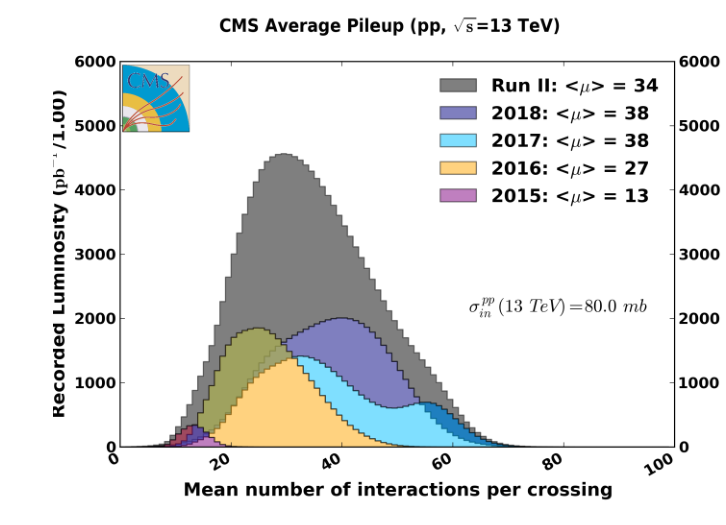
\includegraphics[width=0.49\textwidth]{figures/event_reconstruction/pu.pdf}
    \caption{The average number of vertices per event in CMS during the Run 2 datataking~\cite{CMSlumi}.}
    \label{fig:objreco:pu}
\end{figure}

Track reconstruction describes the process of taking hits from the pixel and strip detectors, combining them and estimating the momentum and flight direction of the charged particle responsible for producing the hits. It is an extremely computationally heavy process and is based on what is called a combinatorial Kalman filter~\cite{BILLOIR1989390}. A Kalman filter is an algorithm that uses time-dependent observations in order to estimate unknown variables, by proceeding progressively from one measurement to the next, improving the knowledge of the
trajectory with each new measurement. The track reconstruction software in CMS (called the Combinatorial Track Finder (CTF)) constructs its collection of tracks by iteratively looping over the hits and reconstructing tracks, then removing those which are already used as inputs for a previous track. It starts from a seed in the inner most tracker layers, usually two or three hits, and then extrapolates the seed trajectories searching for additional hits to associate to that candidate. It then disregards tracks that fail certain criteria  based on a $\chi^2$ calculation taking both hit and trajectory uncertainties into account, as well as the number of missing hits.
The track reconstruction algorithm is effective over the full tracker coverage range up to $|\eta|<2.5$ and can reconstruct particles with momenta as low as 0.1 GeV or particles which are produced up to 60 \cm from the beam line. In the central region, particles with a momentum of 100 GeV have a \PT-resolution of roughly 2.8 \%, a transverse impact parameter resolution of 10 $\micron$ and a longitudinal impact parameter of 30 $\micron$. 


In order to define the location and uncertainty of every proton-proton interaction in an event, primary-vertex reconstruction in performed. Primary vertices lie within a radius of a few millimeters of the beam axis and are defined as the common origin of groups of tracks.
The reconstruction algorithm takes as input the reconstructed tracks from the previous step which pass certain selection criteria, clusters the tracks that share a common origin and then fit for the position of each vertex. Each track must have at least 2 hits in the pixel layers and no less than 5 hits in the pixel+strip as well as a $\chi^2<20$ from a fit to the particle trajectory to be considered as input for the vertex finder. The primary vertex resolution is around 12 \micron in x and 10 \micron in z for vertices with at least 50 tracks.

Offline, all events are required to have at least one primary vertex reconstructed within a 24 \cm window along the beam axis, with a transverse distance from the nominal interaction region of less than 2 \cm. The reconstructed vertex with the largest value of summed physics object $\PT^2$ is selected as the primary interaction vertex where the hard scattering process occurred.

\section{The Particle Flow Algorithm}

After track reconstruction, what remains is an incoherent collection of tracks, calorimeter clusters and hits in the muon chambers. In order to connect these, CMS uses an algorithm called Particle Flow (PF)~\cite{1748-0221-12-10-P10003} to combine the information obtained from all sub-detectors in order to infer which particles were actually produced in the event.
The reconstructed physics object in the order of which they are reconstructed are
\begin{itemize}
  \item Muons, through hits in the tracker and in the muon chambers
  \item Charged hadrons, through hits in the tracker and energy deposits in the calorimeters
  \item Neutral hadrons, through energy deposits in the calorimeters but no hits in the tracker
  \item Photons, through energy deposits in the ECAL but not in the HCAL and no hits in the tracker
  \item Electrons, through hits in the tracker and energy deposits in the ECAL
\end{itemize}

How these different particles propagate through the CMS detector is illustrated in Figure~\ref{fig:objreco:PF}.

\begin{figure}[h] 
    \centering
    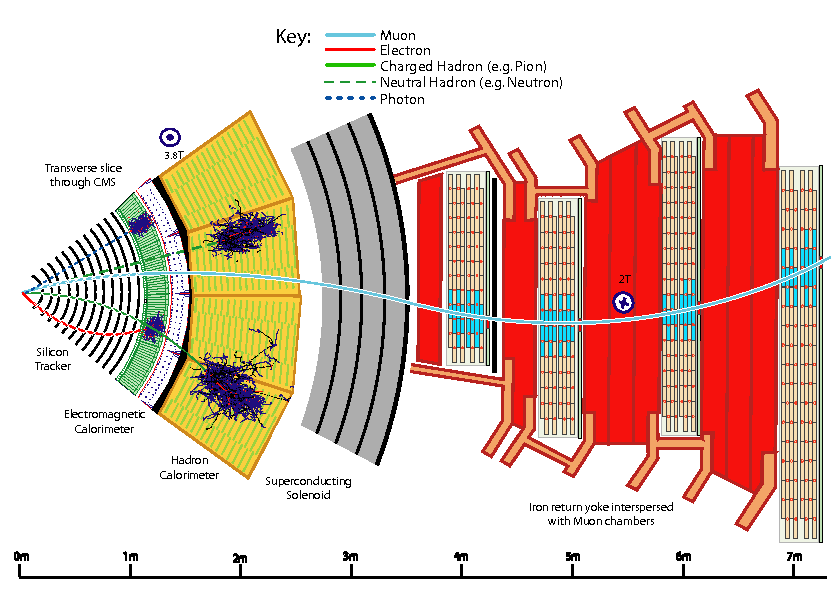
\includegraphics[width=0.79\textwidth]{figures/event_reconstruction/PF.png}
    \caption{Particle interactions in the different subdetectors for a transverse slice through the CMS detector~\cite{1748-0221-12-10-P10003}.}
    \label{fig:objreco:PF}
\end{figure} 

\subsection{Reconstruction of the Particle Flow inputs}

\subsubsection{Electron tracking}
\label{subsub:objreco:electrontracking}
Electron seeding is done in two different ways: ECAL-based  or tracker-based electron seeding. In the ECAL-based method, electrons are seeded from  ECAL clusters with $E_T > 4 \GeV$, where the position of the cluster is used to infer which hits in the inner tracker belongs to a given electron or positron. As a large fraction of the electron/positron energy is emitted through bremsstrahlung before even reaching the ECAL, ECAL superclusters covering a small window in $\eta$ and a larger window in $\phi$ are defined in order to fully contain the electron as well as its bremsstrahlung photons. As these superclusters are prone to contamination, tight isolation requirements need to be applied, leading to reconstruction inefficiencies. Therefore, an additional tracker-based seeding approach has been developed. All tracks with $\PT>2\GeV$ are used as potential electron seeds. These tracks are then extrapolated to the ECAL and matched to the closest ECAL cluster. The ratio of the cluster energy to the track
momentum is required to be ~1. The electron candidates are then fit with a Gaussian-sum filter (GSF)~\cite{0954-3899-31-9-N01} and required to pass certain criteria based on the score of a boosted-decision-tree (BDT) which combines the number of tracker hits, the $\chi^2$ of the GSF track, the energy loss along the  track, and the distance between the extrapolated track to the closest ECAL cluster.

\subsubsection{Muon tracking}
\label{subsub:objreco:muontracking}
Muon tracking consists of two part: the muon spectrometer allows muons to be identified with high efficiency over the full pseudorapidity range, while maintaining a low background due to the absorbing calorimeter layers upstream. The inner tracker on the other hand, provides an accurate measurement of the muon momentum. Three muon quality flags are defined
\begin{itemize}
  \item Standalone muon: Muon tracks based on hits in the DT or CSC only
  \item Global muon: A standalone muon track matched to a track in the tracker if the track parameters of the two are compatible
  \item Tracker muon: An inner track with $\PT> 0.5 \GeV$, a total momentum greater than 2.5 \GeV and at least one muon segment matching the extrapolated inner track
\end{itemize}
Around 99\% of muons produced within $|\eta|<2.4$ are reconstructed as a global muon or a tracker muon, and very often as both. If the global and tracker muon share the same inner tracker segment, the two are combined.

\subsubsection{Calorimeter clusters}
 The calorimeter clustering is performed separately for each calorimeter subdetector (ECAL barrel and endcaps, HCAL barrel and endcaps and the preshower layers).
The first step is to define cluster seeds from cells with an energy exceeding some predefined threshold and in addition is larger than the energy in its neighboring cells. Topological clusters are then formed by adding cells to the seed which has at least one corner in common with a cell already in the cluster, and that has an energy which is at least twice the noise level of the detector. In Figure~\ref{fig:objreco:caloclustering}, an example of calorimeter clustering for a five-particle jet is shown for the HCAL (left) and ECAL (right). In the HCAL (left), two seeds have been identified (gray filled areas) inside a topological cluster consisting of 9 cells. These are then defined as two HCAL clusters, with a position as indicated by the red circles. The green solid lines correspond to charged tracks reconstructed in the tracker, both pointing to the center of the HCAL cluster seeds. The observed deposits left by the same particles are shown on the right in Figure~\ref{fig:objreco:caloclustering}, where the $K^0_L$, $\pi^-$ and the two photons from the decay of a $\pi^0$ leave distinct clusters in the ECAL. The $\pi^+$ leaves no energy deposit in this case. 

\begin{figure}[h] 
    \centering
    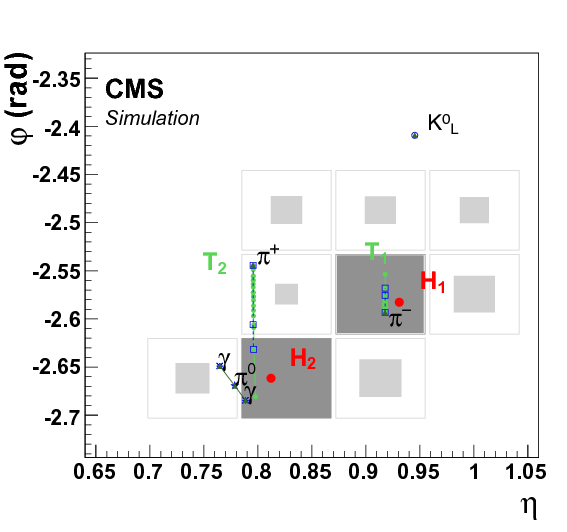
\includegraphics[width=0.49\textwidth]{figures/event_reconstruction/PF_HCAL.png}
    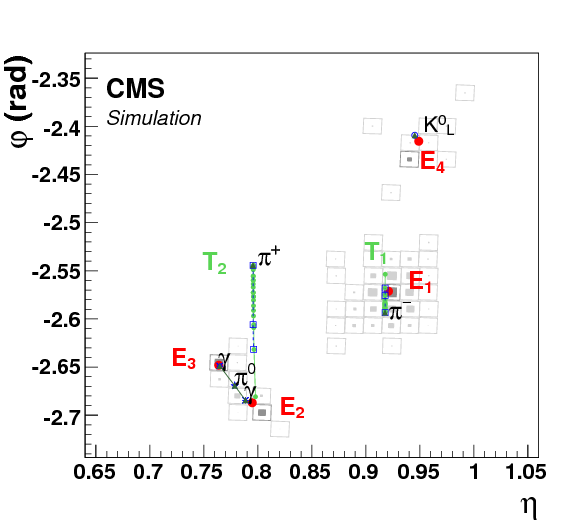
\includegraphics[width=0.49\textwidth]{figures/event_reconstruction/PF_ECAL.png}
    \caption{The $\eta-\phi$ vies of calorimeter clusters generated by a five-particle jet in the HCAL (left) and in the ECAL (right). The squares correspond to calorimeter cells, where the inner area is proportional to the logarith of the cell energy. Cluster seeds are depicted in dark gray. The dotted blue lines correspond to the simulated particle trajectory, while the green lines correspond to charged tracks reconstructed in the tracker~\cite{1748-0221-12-10-P10003}.}
    \label{fig:objreco:caloclustering}
\end{figure} 


\subsection{Particle Flow identification}

\subsubsection{The link algorithm}

The link algorithm is the algorithm responsible for combining the particle flow elements from different subdetectors.
It can test any pair of elements in the event based on specific requirements depending on the nature of the element, but is restricted to the nearest neighbors in the $\eta-\phi$ plane.
The outputs of the link algorithm are so-called \textit{PF blocks} of linked elements, either directly linked or linked through having common elements.
\begin{itemize}
  \item \textbf{Inner track - calorimeter cluster link:} The track is interpolated from its last hit, through the preshower layers, the ECAL and ending in the HCAL at an interaction length depth of 1. A link is made if the track is within the cluster area, where the areas is enlarged by up to a cell in each direction to account for detector gaps. In case several ECAL/HCAL clusters are linked to the same track, only the one with the smallest distance in $\eta-\phi$ is kept.

\item \textbf{Calorimeter cluster - cluster link:} A link between ECAL and HCAL clusters as well as between ECAL and preshower clusters
is made when the cluster position of the more granular calorimeter is within the cluster envelope in the less granular calorimeter. Also here, if there is link overlap, only the link with the smallest distance is kept

\item \textbf{Inner tracker -muon chamber link:} As described in Section~\ref{subsub:objreco:muontracking} 
\end{itemize}

For each PF block, the reconstruction proceeds in the following order.
First, muons are reconstructed and their corresponding PF elements removed from the PF block. Then the electrons are reconstructed, with the hopes of removing their corresponding bremsstrahlung photons from the list of PF elements. Energetic photons are reconstructed in the same step. Finally, neutral and charged hadrons are reconstructed.

\subsubsection{Muons}

First, isolated global muons are selected by requiring the sum of track \PT and calorimeter energy deposits within a cone of $\Delta R = 0.3$ not belonging to the muon track, to be smaller than 10 \% of the muon \PT.
If the muons are non-isolated, they are required to pass the tight muon requirement~\cite{1748-0221-7-10-P10002} and have at least three matching track segments in the muon detector or have matched calorimeter deposits compatible with being a minimum ionizing particle.
Muons failing both the requirements above are kept if the standalone muon track is of high quality and have a lot of hits in the muon detectors, otherwise they are discarded.
The muon momentum is defined from the inner tracker measurement if the muon \PT is less than 200 \GeV. Otherwise, its chosen according to the track fit with the smallest $\chi^2$ probability.

\subsubsection{Electrons}
The electrons are seeded from a GSF track, as described in Section~\ref{subsub:objreco:electrontracking}. To differentiate electrons from charged hadrons, the energy deposit in the HCAL within a distance of 0.15 in the $\eta-\phi$ plane of the supercluster , is required to be less than 10 \% of that of the supercluster. The electron candidate must further pass a requirement on the output of a dedicated electron-identification BDT, using inputs such as track-cluster distance, track $\chi^2$ and number of hits as input.  In this step, isolated photons are also reconstructed, seeded from ECAL superclusters with $|E_T>10 \GeV|$ and no link to a GSF track.
All the tracks and calorimeter deposits used to reconstruct electrons and isolated photons are further removed from the list of PF blocks.

\subsubsection{Hadrons}
Finally, after the removal of muons and electrons, the remaining hadrons and non-isolated photons are identified. HCAL clusters with no track link are defined as neutral hadrons, while ECAL clusters with no track link are defined as photons (photons are exclusively associated to the ECAL deposits as neutral hadrons leave only 3 \% of their energy in the ECAL).
The remaining HCAL clusters are then linked to one or more tracks from the inner tracker. In order to determine the particle content within a cluster, the sum of track momenta and the calorimeter energy is compared.If the calorimeter energy is compatible with the sum of track momenta, a particle for each track is inferred, with its corresponding energy taken from the track momentum.  If the calorimeter energy is larger than the sum of track momenta, a photon or a neutral hadron is added, togehter with one charged hadron for each track within the cluster area.

\section{Pile-up removal}

Particles originating from proton-proton interactions not associated with the hardest primary vertex, are denoted pileup events.
These distorts observables of interest from the hard scattering event and must be mitigated through dedicated pileup removal techniques

\subsection{Charged Hadron Subtraction}
As mentioned previously, primary vertices are reconstructed using tracks from charged hadrons. If a primary vertex does not correspond to the hard scattering vertex of the event, the charged hadrons (as reconstructed through Particle Flow) associated to this vertex (called pileup vertex) are removed from the event collection of particles and will not participate in any further object reconstruction. This method is denoted charged hadron subtraction (CHS).

\subsection{Pile up per particle identification (PUPPI)}
CHS was the default pileup removal algorithm in CMS until very recently. In 2014, a new pileup removal algorithm with improved performance was proposed; the pileup per particle identification (PUPPI)~\cite{Bertolini2014} algorithm.
PUPPI uses a combination of local shape information, event pileup properties and tracking information to compute a weight describing the degree of "pileup-likeness" of a given particle.
First, a variable denoted $\alpha$ is computed based on the difference between soft radiation coming from pileup and the harder collinear QCD pattern. The shape of $\alpha$ for charged particles is then used as a proxy for all pileup particles and is used on an event-by-event basis to calculate a weight for each particle. This weight in turn describes the degree to which particles are pileup-like and are used to rescale the particle four-momenta.

The shape variable for a given particle $i$ is defined as

\begin{equation}
  \alpha_i = \log \sum_{\substack{j \in \mathrm{Ch,PV} \\ j \neq i}} \left(\frac{p_{T,j}}{\Delta R_{ij}}\right)^{2} \Theta(R_0 - \Delta R_{ij}),
\end{equation}

where $\Theta$ is the step function and $j$ refers to the neighboring charged particles from the primary vertex within a cone of radius $R_0=0.4$. Charged particles are defined as coming from the primary vertex if they are associated to the leading vertex of the event or are within a distance of $d_z < $0.3~\cm from the leading vertex. 

In order to determine the probability that a particle comes from pileup, a $\chi^{2}$ calculation is performed. The probability is defined as

\begin{equation}
\chi^{2}_{i} = \frac{(\alpha_i -  \bar{\alpha}_{PU})^{2}}{RMS_{PU}^{2}},
\end{equation}

where $\bar{\alpha}_{PU}$ is the median value of the $\alpha_i$ distribution for pileup particles in the given event and $RMS_{PU}$ is its RMS.

Each particle (neutral and charged) is then assigned a weight $w_i = F_{\chi^2,NDF=1}(\chi^2_i)$, where $F_{\chi^2,NDF=1}$ is the cumulative distribution function of the $\chi^2$ distribution with one degree of freedom. Particles with $w_{i}<0.01$ are rejected.
In addition, a cut on the weighted \PT of neutral particles of $w_{i} \cdot p_{T,i} >  (A + B \cdot N_{PV})$ \GeV is applied, where $N_{PV}$ correspond to the number of reconstructed vertices in the event and A and B are tunable parameters. 

The performance of the PUPPI algorithm compared to CHS for jet observables is shown in Figure~\ref{fig:objreco:puppi}.

\begin{figure}[ht] 
    \centering
    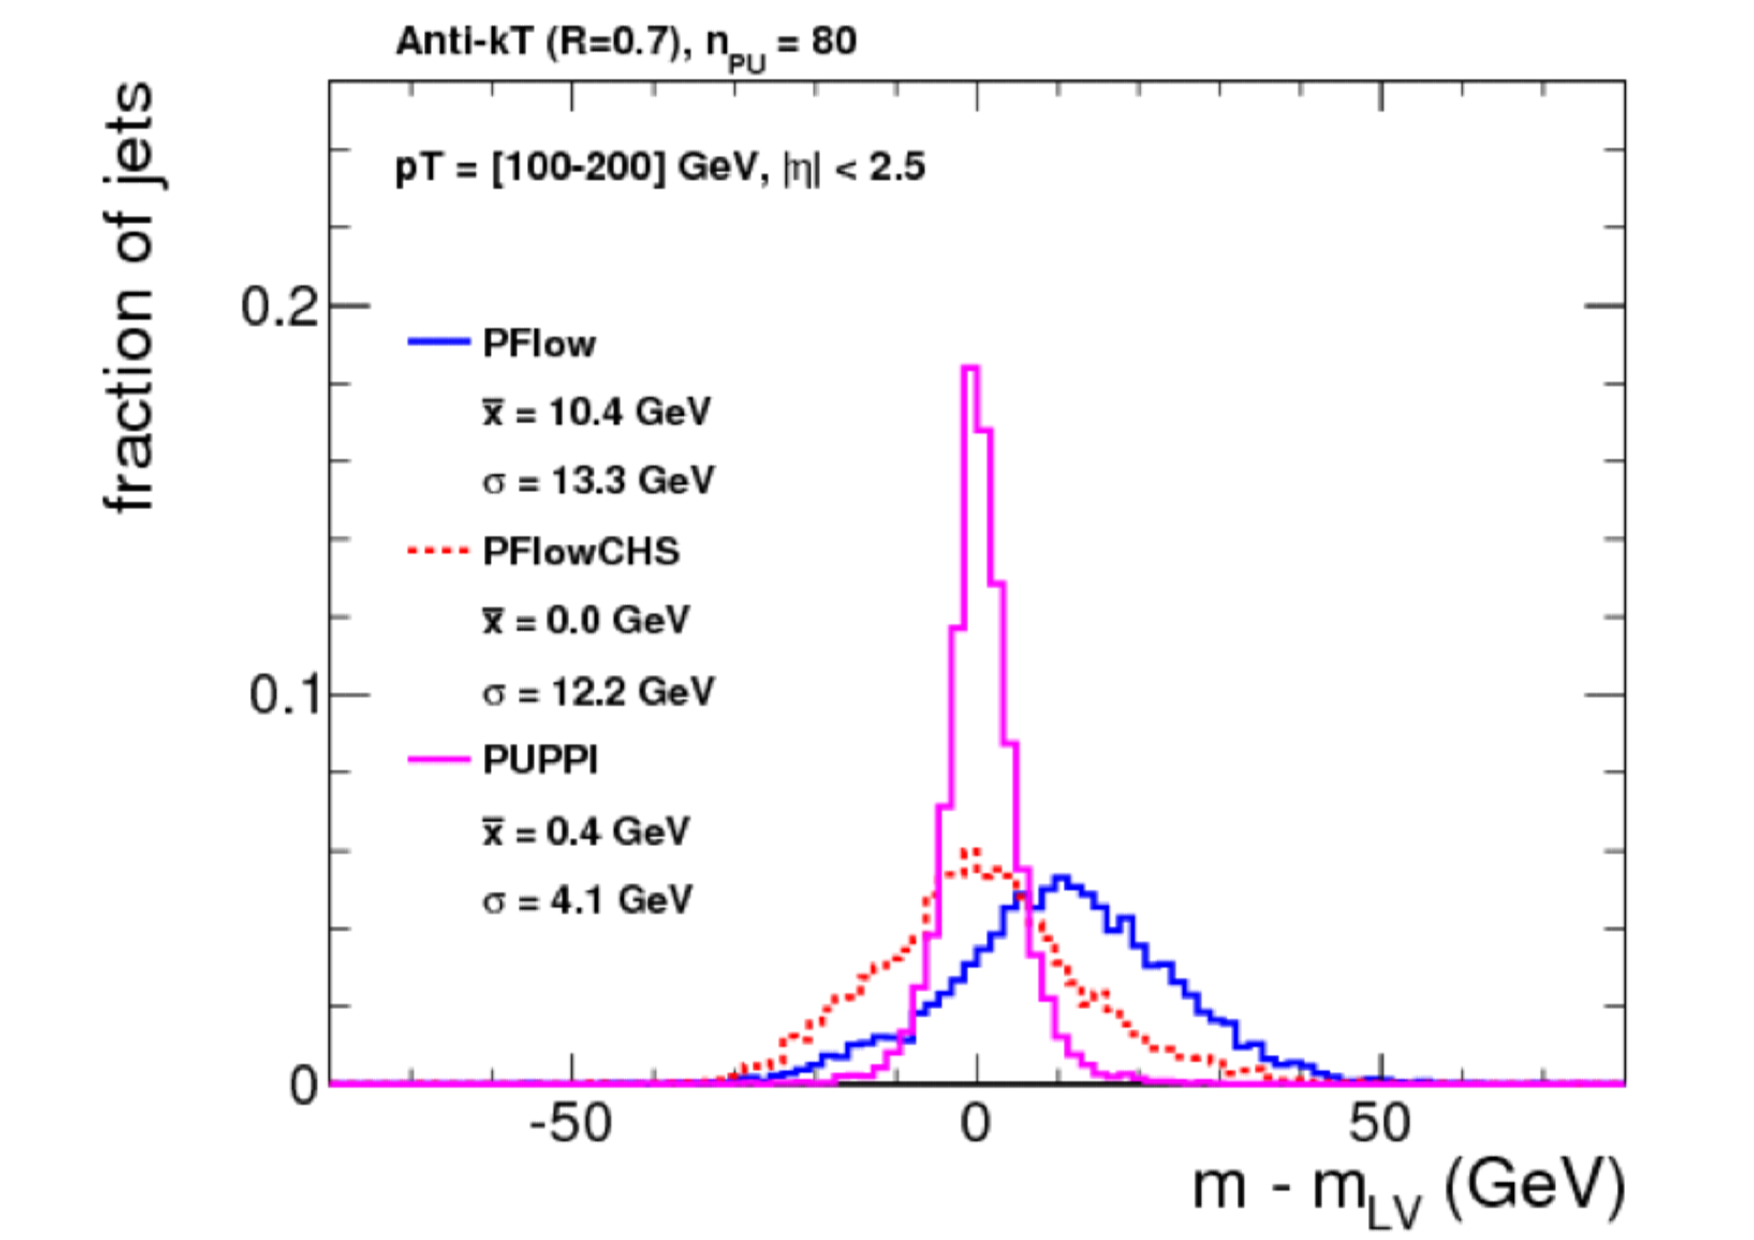
\includegraphics[height=5cm]{figures/event_reconstruction/puppi_mres_hiPt.pdf}
    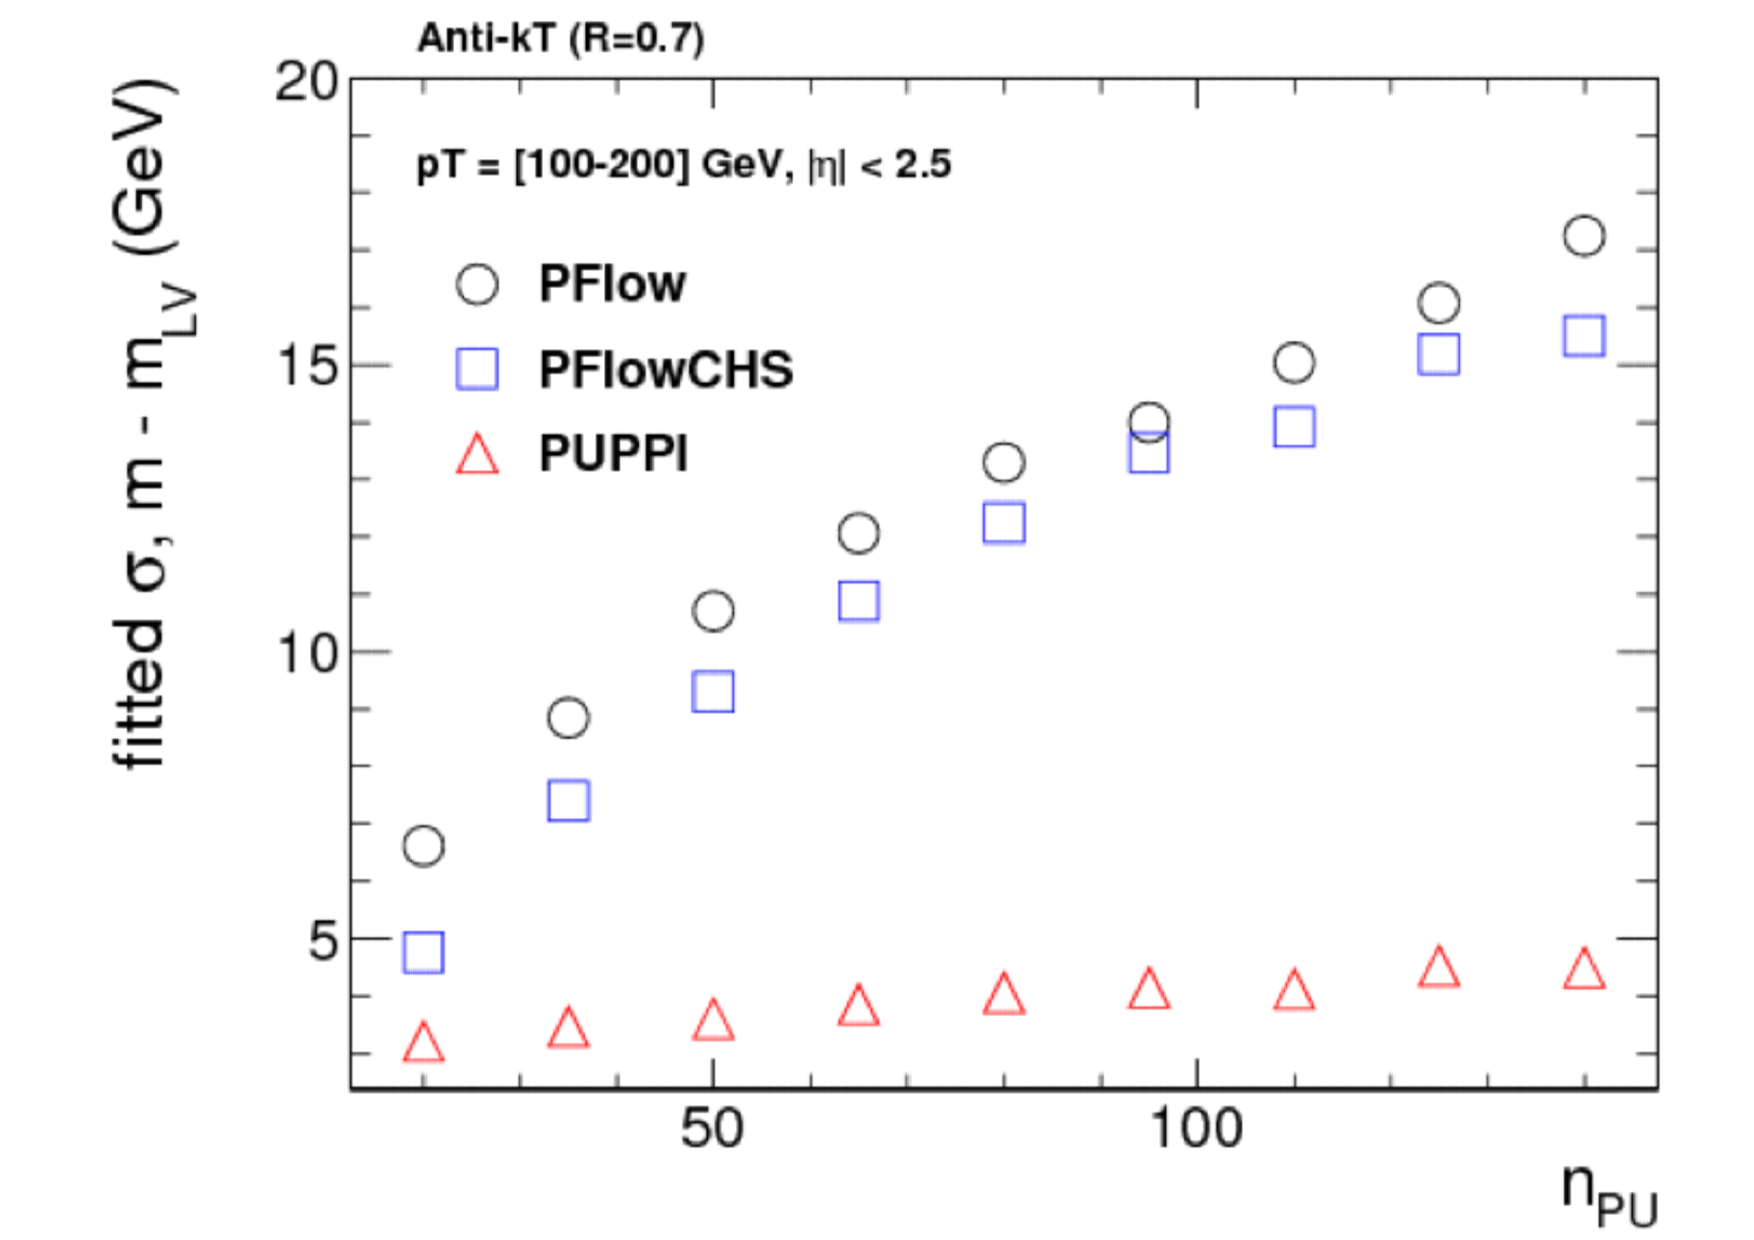
\includegraphics[height=5cm]{figures/event_reconstruction/puppi_mresVsPu.pdf}\\
    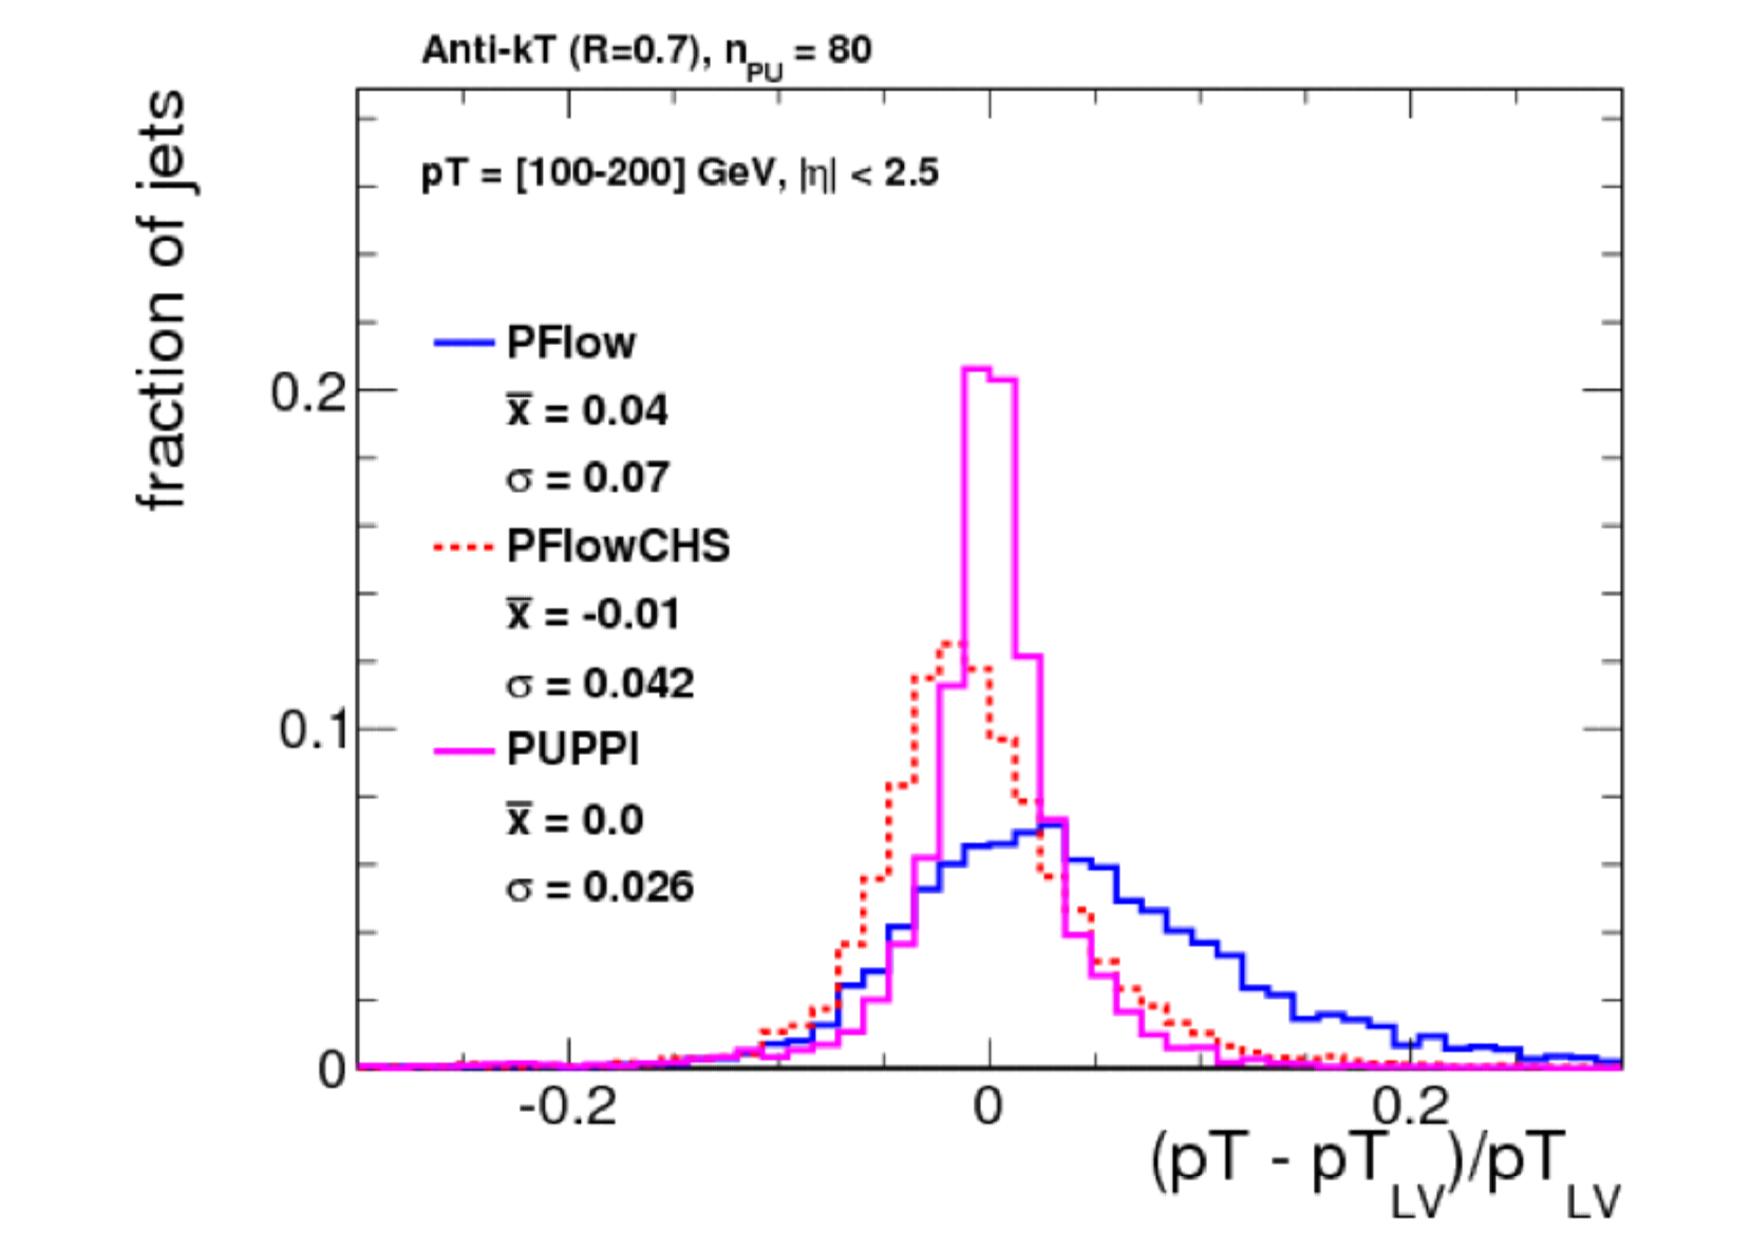
\includegraphics[height=5cm]{figures/event_reconstruction/puppi_ptres_hiPt.pdf}
    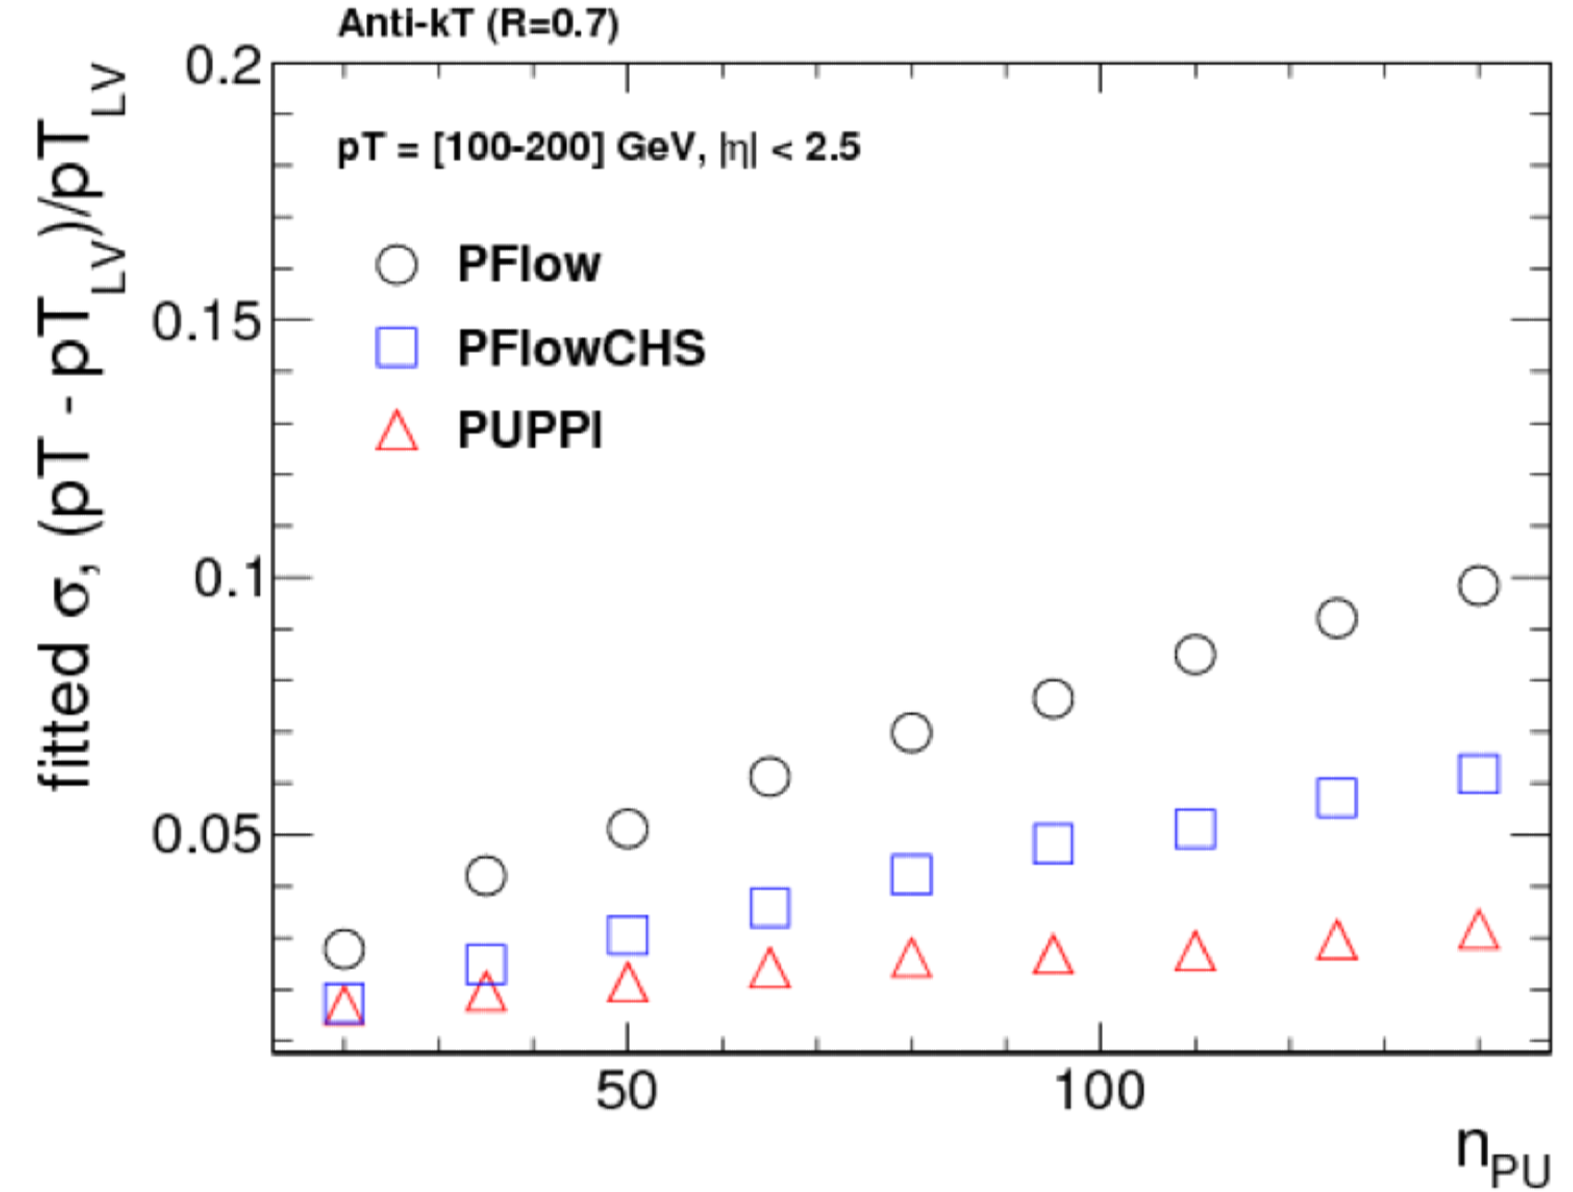
\includegraphics[height=5cm]{figures/event_reconstruction/puppi_ptresVsPu.pdf}
    \caption{The mass (top) and \PT (bottom) resolution comparing PF only (blue), PF+CHS (red) and PUPPI (pink) jets. The absolute resolution (left) as well as the resolution as a function of the number of reconstructed primary vertices in the event (right)is shown~\cite{Bertolini2014}.}
    \label{fig:objreco:puppi}
\end{figure}

The top row shows the absolute mass resolution (left) as well as the mass resolution as a function of $N_{PV}$ for CHS jets (red) and PUPPI (pink) jets. The bottom row shows the corresponding quantities but for jet transverse momentum. A significantly better resolution on jet observables can be achieved using PUPPI compared to CHS.



\section{Jet reconstruction}
As explained in Section~\ref{sec:theory:qcd}, quarks and gluons are never themselves visible in a detector. Within $10^{-23}$ seconds, the timescale of the strong interactions, they fragment and hadronize into a collimated spray of hadrons, a so-called jet. In order to infer the properties of the original parton generating the jet, the properties of the full particle spray needs to be evaluated.
Combining these particles algorithmically is non-trivial, and several algorithms designed to do, called jet clustering algorithms, exist.
These provide a set of rules for grouping particles together into jets and are usually based on certain distance requirements between particles as well as rules for how to recombine their momenta.
Thanks to Particle Flow, objects like charged hadrons, neutral hadrons and photons together with their estimated energy and direction are already defined, and jet clustering in CMS therefore consists of
associating these particles to one common origin.


\subsection{Jet clustering}

The most common jet clustering algorithms used in hadron colliders are the Cambridge/Aachen algorithm~\cite{Dokshitzer:1997in}, the \kt algorithm~\cite{Ellis:1993tq} and the anti-\kt algorithm~\cite{Cacciari:2008gp}. These are all sequential recombination algorithms, meaning they systematically go through each particle pair in the event and recombines them into one particle if the combination satisfies certain criteria. The rules, shared by all three algorithms, are as follows:
\begin{enumerate}
\item For each pair of particles $i$ and $j$, compute the longitudinally invariant distances
  \begin{align}  
  d_{ij} &= \textrm{min}(p_{ti}^{2p},p_{tj}^{2p})\frac{\Delta R^2_{ij}}{R^2} \textrm{, with } \quad \Delta R^2_{ij}&=(\eta_i - \eta_j)^2+(\phi_i - \phi_j)^2\\
  d_{iB} &= p_{ti}^{2p},
  \end{align}  
  where $d_{ij}$ is a measure of the relative transverse momenta between the particles, $\Delta R^2_{ij}$ is the distance between them in the $\eta-\phi$ plane (which can be roughly translated into a jet radius), $\Delta R^2$ corresponds to the desired jet cone size and $d_{iB}$ is the distance between the particle and the beam. The parameter $p$ is what separates the three algorithms from one another. For the anti-\kt algorithm, it is defined as $p=-1$, for the \kt algorithm $p=1$ and in the case of the C/A algorithm, $p=0$. The consequences of these choices are explained in detail below.
  \item Find the minimum distance of $d_{ij}$ and $d_{iB}$.
  \item If this is $d_{ij}$, recombine particles $i$ and $j$ and return to step 1.
  \item If it is $d_{iB}$, the particle is $i$is defined to be a final state jet, and is removed from the list of particles. The algorithms proceeds back to step 1.
  \item Repeat until no particles remain.
\end{enumerate}

\subsubsection{Infrared and collinear safety}
There are two requirements that are extremely important when defining a jet algorithm: It must be 1) infrared and 2) collinear safe.
Infrared safety correspond to the requirement that if the final state particles for some reason are modified by the presence of a soft emission, then the set of hard jets should remain unchanged. This is illustrated in the
found should be unchanged
\subsubsection{The \kt algorithm}
The \kt algorithm is the oldest of the first sequential recombination algorithms. 
\subsubsection{The Cambridge/Aachen algorithm}


\subsubsection{The anti-\kt algorithm}
The default jet clustering algorithm in CMS is the anti-\kt algorithm~\cite{Cacciari:2008gp}, defined through the rules above with $p=-1$. The reason the anti-\kt algorithm is so successful, and the reason why it is used in CMS, is that when using $p=-1$, the algorithm favors the clustering of hard 

%It uses PF candidates as input. Before this clustering occurs, a pileup removal algorithm is applied. If using CHS, charged hadrons not associated to the primary vertex are discarded before clustering. If PUPPI is used, all the PF candidates are reweighted based on how likely they are to have originated from pileup. 

\subsection{Jet substructure reconstruction}
\textcolor{red}{\textbf{TODO!!!}}
\subsubsection{Grooming}
\textcolor{red}{\textbf{TODO!!!}}
\subsubsection{N-subjettiness}
\textcolor{red}{\textbf{TODO!!!}}
\section{Monte Carlo Simulation}
\textcolor{red}{\textbf{TODO!!!}}
\subsection{Matrix Element Generators}
\textcolor{red}{\textbf{TODO!!!}}
\subsection{Shower Generators}
\textcolor{red}{\textbf{TODO!!!}}
